%%%%%% Pfad zum Latex Header
\newcommand{\pfad}{../../../../../../xLatex/x_default/}

\input{\pfad HeadLizenzL.tex}

%%%%% Platz für eigene Imports


%%%%%


%%Variablen Thema der Stunde
\newcommand{\thema}{Herleitung der allgemeinen Tangentengleichung }
%%%%

%%%%%%%%%Header
\begin{document}
	\thispagestyle{specialchapter}
	\parindent 0pt  %% Kein Absatzeinzug
	\vspace*{-1.8cm}
	\hrule 
	\newcolumntype{L}[1]{>{\hsize=#1\hsize\raggedright\arraybackslash}X}%
	\newcolumntype{R}[1]{>{\hsize=#1\hsize\raggedleft\arraybackslash}X}%
	\newcolumntype{C}[1]{>{\hsize=#1\hsize\centering\arraybackslash}X}%
	\begin{tabularx}{\textwidth}{L{0.5} C{2.015} R{0.485}}
		\scriptsize Herr Wienands   & \large \multirow{2}{*}{\textbf{Mathematik}} &  \multirow{3}{*}{\raisebox{-\totalheight}{\includegraphics[scale=0.24]{\pfad Logo.png}}}  \\
		\scriptsize EPH & & \\
		\scriptsize \mydate\today & $\bullet$ \thema $\bullet$ & \\
	\end{tabularx}
	\vspace{0.1cm}
	\hrule
%%%%%%%%%%%%%%%%%%%
\pgfplotsset{compat=1.12}
%%%%%%%%%%%% Plot Settings
\pgfplotsset{every axis/.append style={
		axis x line=middle,    % put the x axis in the middle
		axis y line=middle,    % put the y axis in the middle
		axis line style={->}, % arrows on the axis
		xlabel={$x$},          % default put x on x-axis
		ylabel={$y$},          % default put y on y-axis
	}}\vspace{-0.3cm}
%%%%%%%%%%%%%%%%%%%%%%%%%%%%

	\section*{Problembeschreibung}
		Neben der bekannten Möglichkeit eine Tangente an einer Stelle $x_0$ zu bestimmen gibt es eine weitere. Im Folgenden werden Sie eine allgemeine Formel zur Bestimmung einer Tangentengleichung herleiten.\\
		
		Hierzu bearbeiten Sie die folgende Problemstellung. \\
		\hdashrule{\textwidth}{1pt}{1pt} 
		
		\vspace{0.3cm}
		\begin{minipage}{0.6\textwidth}
			Der Betreiber des Nürburgrings beschließt, nach einem Unfall in einer Kurve, die Pufferzone zu verstärken. Die meisten Unfälle geschehen im Punkt $A(1|2,4)$. Wenn Fahrzeuge an dieser Stelle ausbrechen, dann sollen sie auf eine verbesserte Pufferzone auftreffen. \\
			
			Die Kurve wird durch die Funktion $f(x)=-0,6x^2+2x+1$ beschrieben.\\
			Die vorhandene Pufferzone wird durch die Funktion $p(x)=\frac{1}{3}x+4$ beschrieben. \\
			
			\minisec{Aufgabe 1}
			\begin{enumerate}[a)]
				\item Erstellen Sie eine Skizze im rechten Koordinatensystem.
				\item \textit{Bestimmen Sie zunächst eine Funktion für die ausbrechenden Fahrzeuge ($t(x)$). }
				\item Berechnen Sie die Position der auszubessernden Pufferzone.
			\end{enumerate}

		\end{minipage}
		\begin{minipage}{0.4\textwidth}

			\begin{flushright}
					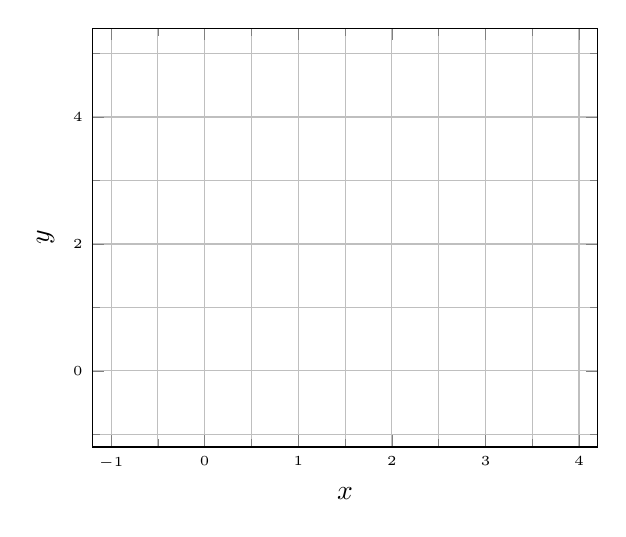
\begin{tikzpicture}
					\begin{axis}[ width=8cm,minor tick num=1, ticklabel style={font=\tiny,fill=white}, xtick={-1,0,1,2,3,4},
					xlabel={$x$},
					ylabel={$y$},xmax=4.2,xmin=-1.2,ymax=5.4,ymin=-1.2,grid=both
					]
					\end{axis}
			\end{tikzpicture}
	
			\end{flushright}
		\end{minipage}
	\hdashrule{\textwidth}{1pt}{1pt} 
	\section*{Entwicklung einer allgemeinen Tangentengleichung}
		\begin{enumerate}[a)]
	\begin{minipage}{0.6\textwidth}
		Die Funktion der ausbrechenden Fahrzeuge soll mithilfe einer Geraden ($t(x)=mx+n$) beschrieben werden.\\ Dabei sind $m$ und $n$ unbekannte. Ihr Ziel ist es diese zu ersetzen.
		\minisec{Aufgabe 2}
			\item Bestimmen Sie $t(x)=mx+n$ mit der Ihnen bekannten Methode und zeichnen Sie diese Funktion in das rechte Koordinatensystem.
			\item Zeichnen Sie in einem ersten Schritt die Funktion $t_1(x)=mx$ in das rechte Koordinatensystem ein.
			\item Ersetzen Sie $m$ in $t_1(x)=mx$ mit einem direkt berechenbaren Ausdruck in Abhängigkeit von $x_0$.
		
		
	\end{minipage}
	\begin{minipage}{0.4\textwidth}
		
		\begin{flushright}
			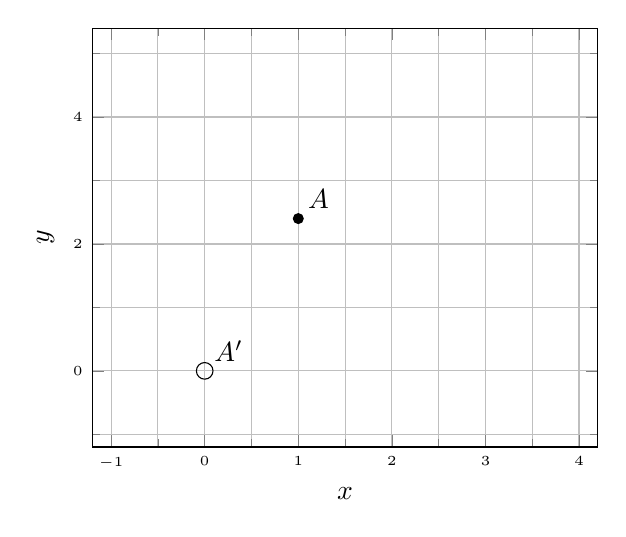
\begin{tikzpicture}
			\begin{axis}[ width=8cm,minor tick num=1, ticklabel style={font=\tiny,fill=white}, xtick={-1,0,1,2,3,4},
			xlabel={$x$},
			ylabel={$y$},xmax=4.2,xmin=-1.2,ymax=5.4,ymin=-1.2,grid=both]
			\draw (0,0) circle[radius=3pt] node[above right] {$A^\prime$};
			\fill (1,2.4) circle[radius=2pt] node[above right] {$A$};
			\end{axis}
			\end{tikzpicture}
			
		\end{flushright}
	\end{minipage}
	\item Vergleichen Sie die beiden Graphen und beschreiben Sie mit eigenen Worten, welche Transformationen durchgeführt werden müssen um $t_1(x)$ in $t(x)$ umzuwandeln. Dabei muss der Punkt $A^\prime$ auf $A$ liegen.
	\item Nutzen Sie Ihr Wissen über Funktionstransformationen und werden Sie die beschriebenen Transformationen auf $t_1(x)$ in Abhängigkeit von $x_0$ an
	\item Notieren Sie Ihre allgemeine Tangentengleichung in den Merkkasten.
\end{enumerate}
\begin{tcolorbox}[title=allgemeine Tangentengleichung]
	\LARGE{$t(x)=$}
\end{tcolorbox}
\end{document}

